\documentclass[11pt,letter,]{article}
\usepackage[margin=1in]{geometry}
\newcommand*{\authorfont}{\fontfamily{phv}\selectfont}
\usepackage[]{mathpazo}
\usepackage{abstract}
\renewcommand{\abstractname}{}    % clear the title
\renewcommand{\absnamepos}{empty} % originally center
\newcommand{\blankline}{\quad\pagebreak[2]}

\providecommand{\tightlist}{%
  \setlength{\itemsep}{0pt}\setlength{\parskip}{0pt}} 
\usepackage{longtable,booktabs}

\usepackage[many]{tcolorbox}
\usepackage{xcolor}
\usepackage{fontawesome5}

% Definición de colores personalizados de Quarto
\definecolor{quarto-callout-note-color-frame}{HTML}{00758A}
\definecolor{quarto-callout-important-color-frame}{HTML}{D41159}
\definecolor{quarto-callout-warning-color-frame}{HTML}{FD8D3C}
\definecolor{quarto-callout-tip-color-frame}{HTML}{00A087}
\definecolor{quarto-callout-caution-color-frame}{HTML}{D41159}
\definecolor{quarto-callout-note-color}{HTML}{00758A}
\definecolor{quarto-callout-important-color}{HTML}{D41159}
\definecolor{quarto-callout-warning-color}{HTML}{FD8D3C}
\definecolor{quarto-callout-tip-color}{HTML}{00A087}
\definecolor{quarto-callout-caution-color}{HTML}{D41159}

\usepackage{parskip}
\usepackage{titlesec}
\titlespacing\section{0pt}{12pt plus 4pt minus 2pt}{6pt plus 2pt minus 2pt}
\titlespacing\subsection{0pt}{12pt plus 4pt minus 2pt}{6pt plus 2pt minus 2pt}

\titleformat*{\subsubsection}{\normalsize\itshape}

\usepackage{hyperref}
\hypersetup{
    colorlinks=true,
    linkcolor=blue,
    filecolor=magenta,      
    urlcolor=blue,
    pdftitle={OPR219: Introducción a las Ciencias Sociales
Computacionales},
    pdfpagemode=FullScreen,
}

\usepackage{titling}
\setlength{\droptitle}{-.25cm}

\usepackage[T1]{fontenc}
\usepackage[utf8]{inputenc}

\usepackage{fancyhdr}
\pagestyle{fancy}
\usepackage{lastpage}
\renewcommand{\headrulewidth}{0.3pt}
\renewcommand{\footrulewidth}{0.0pt} 
\lhead{}
\chead{}
\rhead{\footnotesize OPR219: Introducción a las Ciencias Sociales
Computacionales -- \today}
\lfoot{}
\cfoot{\small \thepage/\pageref*{LastPage}}
\rfoot{}

\fancypagestyle{firststyle}
{
\renewcommand{\headrulewidth}{0pt}%
   \fancyhf{}
   \fancyfoot[C]{\small \thepage/\pageref*{LastPage}}
}

\makeatletter
\@ifpackageloaded{hyperref}{}{%
\ifxetex
  \usepackage[setpagesize=false, % page size defined by xetex
              unicode=false, % unicode breaks when used with xetex
              xetex]{hyperref}
\else
  \usepackage[unicode=true]{hyperref}
\fi
}
\@ifpackageloaded{color}{
    \PassOptionsToPackage{usenames,dvipsnames}{color}
}{%
    \usepackage[usenames,dvipsnames]{color}
}
\makeatother
\hypersetup{breaklinks=true,
            bookmarks=true,
            pdfauthor={ ()},
             pdfkeywords = {},  
            pdftitle={OPR219: Introducción a las Ciencias Sociales
Computacionales},
            colorlinks=true,
            citecolor=blue,
            urlcolor=blue,
            linkcolor=blue,
            pdfborder={0 0 0}}
\urlstyle{same}  % don't use monospace font for urls

\setcounter{secnumdepth}{0}

\usepackage{longtable}

\usepackage{graphicx}
% We will generate all images so they have a width \maxwidth. This means
% that they will get their normal width if they fit onto the page, but
% are scaled down if they would overflow the margins.
\makeatletter
\def\maxwidth{\ifdim\Gin@nat@width>\linewidth\linewidth
\else\Gin@nat@width\fi}
\makeatother
\let\Oldincludegraphics\includegraphics
\renewcommand{\includegraphics}[1]{\Oldincludegraphics[width=\maxwidth]{#1}}


\usepackage{setspace}

\title{OPR219: Introducción a las Ciencias Sociales Computacionales}
\author{Roberto Cantillan}
\date{\today}

\begin{document}  

\maketitle

\thispagestyle{firststyle}

\noindent \begin{tabular*}{\textwidth}{ @{\extracolsep{\fill}} lr @{\extracolsep{\fill}}}
E-mail: \texttt{ricantillan@uc.cl} & Web: Repositorio \href{https://github.com/rcantillan/OPR-219-CIencias-Sociales-Computacionales}{link}\\
Office Hours: Por determinar  &  Class Hours: 10:50 - 14:14\\
Office: Por determinar  & Class Room: J300\\
  &  \\
\hline
\end{tabular*}

\vspace{2mm}

\hypertarget{identificaciuxf3n-de-la-actividad-curricular}{%
\section{Identificación de la Actividad
Curricular}\label{identificaciuxf3n-de-la-actividad-curricular}}

\begin{itemize}
\tightlist
\item
  \textbf{Nombre}: Introducción a las Ciencias Sociales Computacionales
\item
  \textbf{Código}: OPR 219 (Equivalente a SLG-521)
\item
  \textbf{Semestre lectivo}: X
\item
  \textbf{Horas}: Presencial: 54 \textbar{} Autónomas: 96 \textbar{}
  TOTAL: 150
\item
  \textbf{Créditos SCT}: 5
\item
  \textbf{Duración}: Semestral
\item
  \textbf{Modalidad}: Presencial
\item
  \textbf{Área de Formación}: Profesional
\item
  \textbf{Requisito}: Todas las actividades curriculares aprobadas hasta
  el VIII semestre
\end{itemize}

\hypertarget{descripciuxf3n-y-caracterizaciuxf3n-de-la-actividad-curricular}{%
\section{Descripción y Caracterización de la Actividad
Curricular}\label{descripciuxf3n-y-caracterizaciuxf3n-de-la-actividad-curricular}}

La actividad curricular de Electivo II Ciencias Sociales Computacionales
se ubica en el X semestre de la carrera de Sociología y pertenece al
área de formación profesional.

En la era actual, caracterizada por la abundancia de datos digitales y
nuevas herramientas computacionales, las ciencias sociales se encuentran
en un punto de inflexión que ofrece oportunidades sin precedentes para
el estudio del comportamiento social. Este curso tiene como propósito
central explorar y evaluar el impacto transformador de los avances
tecnológicos en la investigación social, con un enfoque particular en la
transición de métodos analógicos a digitales.

Durante el curso, realizaremos una revisión exhaustiva de las
principales oportunidades y ventajas que se abren en la era digital para
quienes estudian el comportamiento social. Esto incluirá un análisis
detallado de las nuevas fuentes de datos y métodos, como el análisis de
texto a gran escala, el estudio de contenidos multimedia, y la
exploración de datos de redes sociales. Examinaremos cómo estas nuevas
fuentes de datos y métodos están cambiando no solo las respuestas que
podemos obtener, sino también las preguntas que podemos formular en las
ciencias sociales.

Un componente clave del curso será el ejercicio de imaginar y formular
problemas sustantivos a partir de datos producidos digitalmente. Este
enfoque nos permitirá explorar cómo los conceptos tradicionales de
diseño de investigación en las ciencias sociales pueden aplicarse y
adaptarse para analizar estas nuevas fuentes de datos. Al mismo tiempo,
consideraremos cómo estas nuevas fuentes de datos pueden requerir una
reevaluación y adaptación de nuestros enfoques tradicionales de diseño
de investigación.

El curso también abordará los desafíos éticos y metodológicos que surgen
con el uso de big data y métodos computacionales en las ciencias
sociales. Discutiremos temas como la privacidad, el consentimiento
informado en la era digital, y las implicaciones de la brecha digital en
la representatividad de nuestros datos y resultados.

La metodología de enseñanza-aprendizaje incluirá clases expositivas,
revisión de material bibliográfico, aplicación de técnicas de Design
Thinking, y un enfoque de Aprendizaje Basado en Proyectos. La evaluación
se basará en la elaboración de un proyecto de investigación, cuyos
avances se presentarán mediante informes escritos y exposiciones orales.
Además, se incorporarán elementos de coevaluación y autoevaluación para
fomentar la reflexión crítica sobre el propio proceso de aprendizaje.

Este curso requiere un compromiso activo por parte de los estudiantes.
En su tiempo autónomo, deberán realizar lecturas, participar en trabajos
colaborativos, y buscar de forma independiente ejemplos de investigación
en el área que complementen los presentados en clase y que puedan ser
útiles para el desarrollo de su proyecto.

Al finalizar el curso, los estudiantes habrán desarrollado una
comprensión profunda de cómo la revolución digital está transformando
las ciencias sociales, y estarán equipados con las habilidades
necesarias para aprovechar estas nuevas oportunidades en su futura
carrera profesional o académica.

\hypertarget{competencias-del-perfil-de-egreso-asociadas-a-la-actividad-curricular}{%
\section{Competencias del Perfil de Egreso Asociadas a la Actividad
Curricular}\label{competencias-del-perfil-de-egreso-asociadas-a-la-actividad-curricular}}

\hypertarget{competencias-profesionales}{%
\subsection{Competencias
Profesionales}\label{competencias-profesionales}}

\begin{enumerate}
\def\labelenumi{\arabic{enumi}.}
\tightlist
\item
  Gestionar organizaciones, proyectos e intervenciones orientándose al
  trabajo colaborativo y con apertura a la diversidad social.

  \begin{itemize}
  \tightlist
  \item
    1.3. Gestionar proyectos e intervenciones sociales, promoviendo el
    trabajo en equipo interdisciplinar y colaborativo.
  \end{itemize}
\item
  Proponer iniciativas pertinentes a las demandas y necesidades de
  entidades diversas, en base a una comprensión integral de los
  fenómenos y los contextos sociales.

  \begin{itemize}
  \tightlist
  \item
    2.3. Proponer iniciativas pertinentes, relacionando críticamente
    conceptos y teorías contemporáneas de la sociología y las ciencias
    sociales.
  \end{itemize}
\end{enumerate}

\hypertarget{competencias-genuxe9ricas}{%
\subsection{Competencias Genéricas}\label{competencias-genuxe9ricas}}

\begin{enumerate}
\def\labelenumi{\arabic{enumi}.}
\tightlist
\item
  Realizar investigaciones que contribuyan al desarrollo del
  conocimiento científico y aplicado en contextos propios de su proceso
  formativo.

  \begin{itemize}
  \tightlist
  \item
    1.1. Desarrollar investigación aplicada, implementando los pasos del
    método científico y articulando conclusiones adecuadas y coherentes
    al proceso investigativo.
  \end{itemize}
\end{enumerate}

\hypertarget{resultados-de-aprendizaje---aprendizajes-esperados}{%
\section{Resultados de Aprendizaje - Aprendizajes
Esperados}\label{resultados-de-aprendizaje---aprendizajes-esperados}}

\begin{enumerate}
\def\labelenumi{\arabic{enumi}.}
\tightlist
\item
  Analizar las ventajas y obstáculos que presenta la era digital en el
  contexto de la investigación social, considerando aspectos de ética
  científica y las implicaciones metodológicas del uso de big data.
\item
  Diseñar propuestas de investigación aplicada integrando conceptos de
  las ciencias sociales y la ciencia de datos, promoviendo el trabajo
  colaborativo y aprovechando las nuevas fuentes de datos digitales.
\item
  Evaluar críticamente las implicaciones éticas y sociales del uso de
  métodos computacionales y big data en la investigación social.
\item
  Desarrollar habilidades para la formulación de preguntas de
  investigación innovadoras utilizando datos producidos digitalmente.
\end{enumerate}

\hypertarget{unidades-de-aprendizaje-y-ejes-temuxe1ticos}{%
\section{Unidades de Aprendizaje y Ejes
Temáticos}\label{unidades-de-aprendizaje-y-ejes-temuxe1ticos}}

\hypertarget{semana-01-0808---1208-introducciuxf3n-a-las-ciencias-sociales-computacionales}{%
\subsection{Semana 01, 08/08 - 12/08: Introducción a las Ciencias
Sociales
Computacionales}\label{semana-01-0808---1208-introducciuxf3n-a-las-ciencias-sociales-computacionales}}

\begin{itemize}
\tightlist
\item
  Trayectoria y evolución de las ciencias sociales computacionales
\item
  Oportunidades y desafíos de la revolución digital en las ciencias
  sociales
\item
  Nuevas preguntas y métodos en la era del big data
\end{itemize}

\hypertarget{semana-02-1508---1908-jueves-15-de-agosto---feriado-asunciuxf3n-de-la-virgen}{%
\subsection{Semana 02, 15/08 - 19/08: Jueves 15 de Agosto - Feriado
(Asunción de la
Virgen)}\label{semana-02-1508---1908-jueves-15-de-agosto---feriado-asunciuxf3n-de-la-virgen}}

\begin{itemize}
\tightlist
\item
  No hay clases
\end{itemize}

\hypertarget{semana-03-2208---2608-fundamentos-de-datos-digitales}{%
\subsection{Semana 03, 22/08 - 26/08: Fundamentos de Datos
Digitales}\label{semana-03-2208---2608-fundamentos-de-datos-digitales}}

\begin{itemize}
\tightlist
\item
  Tipos de datos digitales: textuales, de red, geoespaciales, de
  comportamiento
\item
  Características y potencial de los datos digitales en la investigación
  social
\item
  Introducción a las fuentes de datos digitales para las ciencias
  sociales
\end{itemize}

\hypertarget{semana-04-2908---0209-diseuxf1o-de-investigaciuxf3n-en-la-era-digital-i}{%
\subsection{Semana 04, 29/08 - 02/09: Diseño de Investigación en la Era
Digital
I}\label{semana-04-2908---0209-diseuxf1o-de-investigaciuxf3n-en-la-era-digital-i}}

\begin{itemize}
\tightlist
\item
  Adaptación de métodos tradicionales al contexto digital
\item
  Estrategias de muestreo y representatividad en datos digitales
\item
  Ética en la investigación con datos digitales
\end{itemize}

\hypertarget{semana-05-0509---0909-diseuxf1o-de-investigaciuxf3n-en-la-era-digital-ii}{%
\subsection{Semana 05, 05/09 - 09/09: Diseño de Investigación en la Era
Digital
II}\label{semana-05-0509---0909-diseuxf1o-de-investigaciuxf3n-en-la-era-digital-ii}}

\begin{itemize}
\tightlist
\item
  Experimentos en línea y A/B testing
\item
  Encuestas digitales y nuevas formas de recolección de datos
\item
  Métodos de colaboración masiva y ciencia ciudadana
\end{itemize}

\hypertarget{semana-06-1209---1609-anuxe1lisis-de-texto-y-contenido-digital}{%
\subsection{Semana 06, 12/09 - 16/09: Análisis de Texto y Contenido
Digital}\label{semana-06-1209---1609-anuxe1lisis-de-texto-y-contenido-digital}}

\begin{itemize}
\tightlist
\item
  Introducción al análisis de contenido digital
\item
  Potencial y limitaciones del análisis de texto a gran escala
\item
  Consideraciones metodológicas en el análisis de contenido en línea
\end{itemize}

\hypertarget{semana-07-1909---2309-semana-del-18-de-septiembre---feriado-fiestas-patrias}{%
\subsection{Semana 07, 19/09 - 23/09: Semana del 18 de Septiembre -
Feriado (Fiestas
Patrias)}\label{semana-07-1909---2309-semana-del-18-de-septiembre---feriado-fiestas-patrias}}

\begin{itemize}
\tightlist
\item
  No hay clases
\end{itemize}

\hypertarget{semana-08-2609---3009-anuxe1lisis-de-redes-sociales}{%
\subsection{Semana 08, 26/09 - 30/09: Análisis de Redes
Sociales}\label{semana-08-2609---3009-anuxe1lisis-de-redes-sociales}}

\begin{itemize}
\tightlist
\item
  Conceptos fundamentales de análisis de redes
\item
  Redes sociales digitales como fuente de datos
\item
  Implicaciones teóricas y metodológicas del análisis de redes sociales
  digitales
\end{itemize}

\hypertarget{semana-09-0310---0710-aprendizaje-automuxe1tico-en-ciencias-sociales}{%
\subsection{Semana 09, 03/10 - 07/10: Aprendizaje Automático en Ciencias
Sociales}\label{semana-09-0310---0710-aprendizaje-automuxe1tico-en-ciencias-sociales}}

\begin{itemize}
\tightlist
\item
  Introducción conceptual al aprendizaje automático
\item
  Aplicaciones potenciales en la investigación social
\item
  Desafíos y consideraciones éticas del uso de IA en ciencias sociales
\end{itemize}

\hypertarget{semana-10-1010---1410-visualizaciuxf3n-de-datos-y-comunicaciuxf3n-de-resultados}{%
\subsection{Semana 10, 10/10 - 14/10: Visualización de Datos y
Comunicación de
Resultados}\label{semana-10-1010---1410-visualizaciuxf3n-de-datos-y-comunicaciuxf3n-de-resultados}}

\begin{itemize}
\tightlist
\item
  Principios de visualización efectiva de datos
\item
  Narrativa de datos y presentación de resultados de investigación
\item
  Ética en la visualización y comunicación de datos
\end{itemize}

\hypertarget{semana-11-1710---2110-uxe9tica-y-responsabilidad-en-las-ciencias-sociales-computacionales}{%
\subsection{Semana 11, 17/10 - 21/10: Ética y Responsabilidad en las
Ciencias Sociales
Computacionales}\label{semana-11-1710---2110-uxe9tica-y-responsabilidad-en-las-ciencias-sociales-computacionales}}

\begin{itemize}
\tightlist
\item
  Privacidad y protección de datos en la investigación digital
\item
  Sesgo algorítmico y equidad en el análisis computacional
\item
  Implicaciones sociales y políticas del big data en las ciencias
  sociales
\end{itemize}

\hypertarget{semana-12-2410---2810-proyecto-de-investigaciuxf3n---desarrollo}{%
\subsection{Semana 12, 24/10 - 28/10: Proyecto de Investigación -
Desarrollo}\label{semana-12-2410---2810-proyecto-de-investigaciuxf3n---desarrollo}}

\begin{itemize}
\tightlist
\item
  Definición de temas de investigación
\item
  Formación de equipos y planificación de proyectos
\item
  Asesorías y trabajo guiado en los proyectos
\end{itemize}

\hypertarget{semana-13-3110---0411-viernes-1-de-noviembre---feriado-duxeda-de-todos-los-santos}{%
\subsection{Semana 13, 31/10 - 04/11: Viernes 1 de Noviembre - Feriado
(Día de Todos los
Santos)}\label{semana-13-3110---0411-viernes-1-de-noviembre---feriado-duxeda-de-todos-los-santos}}

\begin{itemize}
\tightlist
\item
  No hay clases
\end{itemize}

\hypertarget{semana-14-0711---1111-proyecto-de-investigaciuxf3n---continuaciuxf3n}{%
\subsection{Semana 14, 07/11 - 11/11: Proyecto de Investigación -
Continuación}\label{semana-14-0711---1111-proyecto-de-investigaciuxf3n---continuaciuxf3n}}

\begin{itemize}
\tightlist
\item
  Trabajo en equipo sobre propuestas de investigación
\item
  Asesorías individuales
\end{itemize}

\hypertarget{semana-15-1411---1811-presentaciones-de-avance}{%
\subsection{Semana 15, 14/11 - 18/11: Presentaciones de
Avance}\label{semana-15-1411---1811-presentaciones-de-avance}}

\begin{itemize}
\tightlist
\item
  Exposiciones orales de los avances de proyectos
\item
  Retroalimentación grupal
\end{itemize}

\hypertarget{semana-16-2111---2511-proyecto-de-investigaciuxf3n---finalizaciuxf3n}{%
\subsection{Semana 16, 21/11 - 25/11: Proyecto de Investigación -
Finalización}\label{semana-16-2111---2511-proyecto-de-investigaciuxf3n---finalizaciuxf3n}}

\begin{itemize}
\tightlist
\item
  Incorporación de retroalimentación
\item
  Preparación de informes finales
\end{itemize}

\hypertarget{semana-17-2811---0212-presentaciones-finales}{%
\subsection{Semana 17, 28/11 - 02/12: Presentaciones
Finales}\label{semana-17-2811---0212-presentaciones-finales}}

\begin{itemize}
\tightlist
\item
  Exposiciones orales de los proyectos finales
\item
  Evaluación y cierre del curso
\end{itemize}

\hypertarget{estrategias-de-enseuxf1anza-y-aprendizaje}{%
\section{Estrategias de Enseñanza y
Aprendizaje}\label{estrategias-de-enseuxf1anza-y-aprendizaje}}

\begin{itemize}
\tightlist
\item
  Clases expositivas dialogadas
\item
  Aprendizaje Basado en Proyectos
\item
  Design Thinking
\item
  Discusiones grupales y debates éticos
\item
  Tutorías y asesorías individuales para proyectos
\end{itemize}

\hypertarget{evaluaciuxf3n}{%
\section{Evaluación}\label{evaluaciuxf3n}}

\hypertarget{propuesta-de-investigaciuxf3n-inicial-y-presentaciuxf3n-30}{%
\subsection{Propuesta de Investigación Inicial y Presentación
(30\%)}\label{propuesta-de-investigaciuxf3n-inicial-y-presentaciuxf3n-30}}

\hypertarget{instrumento}{%
\subsubsection{Instrumento}\label{instrumento}}

Rúbrica e Informe (Escala de apreciación)

\hypertarget{contenidos-y-ponderaciuxf3n}{%
\subsubsection{Contenidos y
Ponderación}\label{contenidos-y-ponderaciuxf3n}}

\begin{itemize}
\tightlist
\item
  Identificación y justificación del problema de investigación (25\%)
\item
  Revisión preliminar de literatura relevante (25\%)
\item
  Formulación de preguntas de investigación innovadoras (30\%)
\item
  Consideración de aspectos éticos en la investigación social
  computacional (20\%)
\end{itemize}

\hypertarget{formato}{%
\subsubsection{Formato}\label{formato}}

\begin{itemize}
\tightlist
\item
  Informe escrito (máximo 2000 palabras)
\item
  Presentación oral (10 minutos)
\end{itemize}

\hypertarget{diseuxf1o-metodoluxf3gico-y-estrategia-de-recolecciuxf3n-de-datos-40}{%
\subsection{Diseño Metodológico y Estrategia de Recolección de Datos
(40\%)}\label{diseuxf1o-metodoluxf3gico-y-estrategia-de-recolecciuxf3n-de-datos-40}}

\hypertarget{instrumento-1}{%
\subsubsection{Instrumento}\label{instrumento-1}}

Rúbrica y Autoevaluación de proceso

\hypertarget{contenidos-y-ponderaciuxf3n-1}{%
\subsubsection{Contenidos y
Ponderación}\label{contenidos-y-ponderaciuxf3n-1}}

\begin{itemize}
\tightlist
\item
  Propuesta metodológica innovadora (30\%)
\item
  Identificación y justificación de fuentes de datos diversas (25\%)
\item
  Estrategia de recolección y procesamiento de datos (25\%)
\item
  Consideraciones éticas y de privacidad en la recolección de datos
  (20\%)
\end{itemize}

\hypertarget{formato-1}{%
\subsubsection{Formato}\label{formato-1}}

\begin{itemize}
\tightlist
\item
  Informe de avance (máximo 2500 palabras)
\item
  Sesión de retroalimentación grupal
\end{itemize}

\hypertarget{proyecto-final-diseuxf1o-completo-de-investigaciuxf3n-30}{%
\subsection{Proyecto Final: Diseño Completo de Investigación
(30\%)}\label{proyecto-final-diseuxf1o-completo-de-investigaciuxf3n-30}}

\hypertarget{instrumento-2}{%
\subsubsection{Instrumento}\label{instrumento-2}}

Rúbrica de evaluación de proyecto y presentación

\hypertarget{contenidos-y-ponderaciuxf3n-2}{%
\subsubsection{Contenidos y
Ponderación}\label{contenidos-y-ponderaciuxf3n-2}}

\begin{itemize}
\tightlist
\item
  Refinamiento de preguntas de investigación y justificación teórica
  (20\%)
\item
  Diseño metodológico detallado (25\%)
\item
  Plan de análisis de datos (25\%)
\item
  Discusión de limitaciones y consideraciones éticas (15\%)
\item
  Propuesta de difusión y aplicación de resultados (15\%)
\end{itemize}

\hypertarget{formato-2}{%
\subsubsection{Formato}\label{formato-2}}

\begin{itemize}
\tightlist
\item
  Informe final (máximo 4000 palabras)
\item
  Presentación (15 minutos)
\end{itemize}

\begin{figure}

{\centering 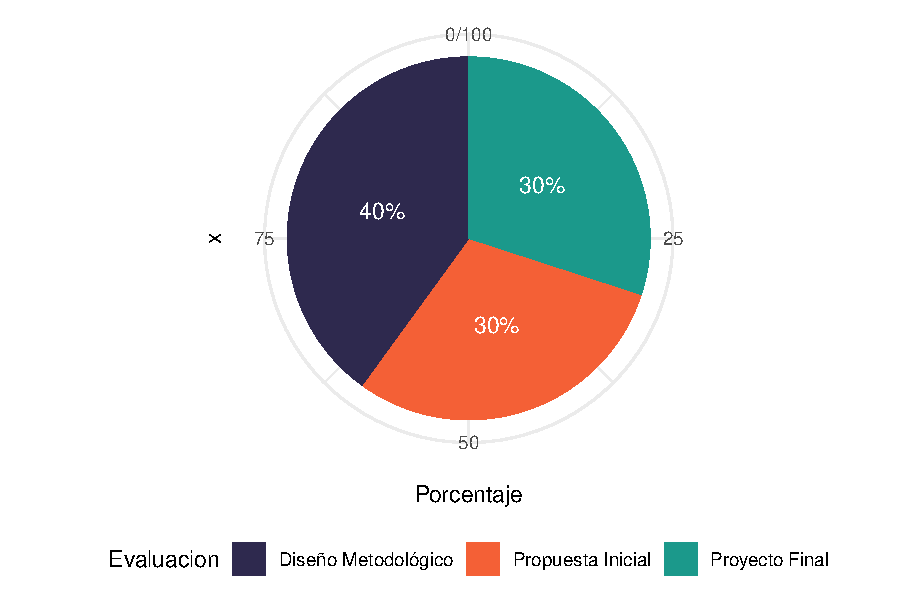
\includegraphics{programa_files/figure-pdf/unnamed-chunk-1-1.pdf}

}

\caption{Distribución de la evaluación del curso}

\end{figure}

\hypertarget{notas-adicionales}{%
\section{Notas Adicionales}\label{notas-adicionales}}

\begin{tcolorbox}[enhanced jigsaw, coltitle=black, rightrule=.15mm, breakable, opacitybacktitle=0.6, opacityback=0, bottomrule=.15mm, colback=white, arc=.35mm, colbacktitle=quarto-callout-note-color!10!white, left=2mm, toprule=.15mm, titlerule=0mm, bottomtitle=1mm, toptitle=1mm, leftrule=.75mm, title=\textcolor{quarto-callout-note-color}{\faInfo}\hspace{0.5em}{Note}, colframe=quarto-callout-note-color-frame]

\begin{itemize}
\tightlist
\item
  Se incentiva el pensamiento creativo y la propuesta de métodos
  innovadores que combinen diferentes fuentes de datos.
\item
  La evaluación se centrará en la calidad del diseño de investigación
  más que en la aplicación práctica.
\item
  Se valorará especialmente la justificación teórica sólida y la
  alineación entre las preguntas de investigación y la metodología
  propuesta.
\item
  Los estudiantes deben considerar fuentes de datos no convencionales y
  explicar cómo las utilizarían en un escenario ideal.
\end{itemize}

\end{tcolorbox}

\hypertarget{recursos-de-infraestructura}{%
\section{Recursos de
Infraestructura}\label{recursos-de-infraestructura}}

\begin{itemize}
\tightlist
\item
  Sala de clases con proyector y audio
\item
  Laboratorio de computación con R y RStudio instalado
\item
  Acceso a UCM Virtual (Plataforma Web LMS)
\item
  Acceso a bases de datos y repositorios de datos abiertos
\end{itemize}

\hypertarget{recursos-bibliogruxe1ficos}{%
\section{Recursos Bibliográficos}\label{recursos-bibliogruxe1ficos}}

\hypertarget{buxe1sica-obligatoria}{%
\subsection{Básica Obligatoria}\label{buxe1sica-obligatoria}}

\begin{itemize}
\tightlist
\item
  Salganik, Matthew J. (2017). Bit by Bit: Social Research in the
  Digital Age. Princeton, NJ: Princeton University Press. Open review
  edition. Versión online \url{https://www.bitbybitbook.com/}.
\item
  Ismay, C., \& Kim, A. Y.-S. (2020). Statistical inference via data
  science: A ModernDive into R and the Tidyverse. CRC Press / Taylor \&
  Francis Group. (versión gitbook de libre acceso:
  \url{https://moderndive.com/})
\end{itemize}

\hypertarget{complementaria}{%
\subsection{Complementaria}\label{complementaria}}

\begin{itemize}
\tightlist
\item
  Imai, K., \& Williams, N. W. (2022). Quantitative Social Science: An
  Introduction in Tidyverse. Princeton University Press.
\item
  Edelmann, A., Wolff, T., Montagne, D., \& Bail, C. A. (2020).
  Computational Social Science and Sociology. Annual Review of
  Sociology, 46(1), 61--81.
  \url{https://doi.org/10.1146/annurev-soc-121919-054621}
\item
  Buyalskaya, A., Gallo, M., \& Camerer, C. F. (2021). The golden age of
  social science. Proceedings of the National Academy of Sciences,
  118(5), e2002923118. \url{https://doi.org/10.1073/pnas.2002923118}
\item
  Lazer, D., Pentland, A., Adamic, L., Aral, S., Barabási, A.-L.,
  Brewer, D., Christakis, N., Contractor, N., Fowler, J., Gutmann, M.,
  Jebara, T., King, G., Macy, M., Roy, D., \& Van Alstyne, M. (2009).
  Computational Social Science. Science, 323(5915), 721--723.
  \url{https://doi.org/10.1126/science.1167742}
\item
  Wickham, H., Çetinkaya-Rundel, M., \& Grolemund, G. (2023). R for data
  science. O'Reilly Media, Inc.~Versión en español: R para ciencia de
  datos: \url{https://es.r4ds.hadley.nz/}
\item
  Wickham, H. (2019). Advanced r. CRC press. (link a versión on line de
  libre acceso {[}https://adv-r.hadley.nz/{]}(https://
\end{itemize}

\end{document}

\makeatletter
\def\@maketitle{%
  \newpage
  \let \footnote \thanks
    {\fontsize{18}{20}\selectfont\raggedright  \setlength{\parindent}{0pt} \@title \par}%
}
\makeatother
